\section{Gallery}
\label{sec:vis_gallery}
A picture is worth a thousand words. In this section we will show some screen shots from the visualization tool we have made. The DSMC visualizer can both render the state of the system while it integrates the system forward in time - a live visualization. This makes it easier to find interesting regions in the system, or is great as a show-off case.

\begin{figure}[htb]
\begin{center}
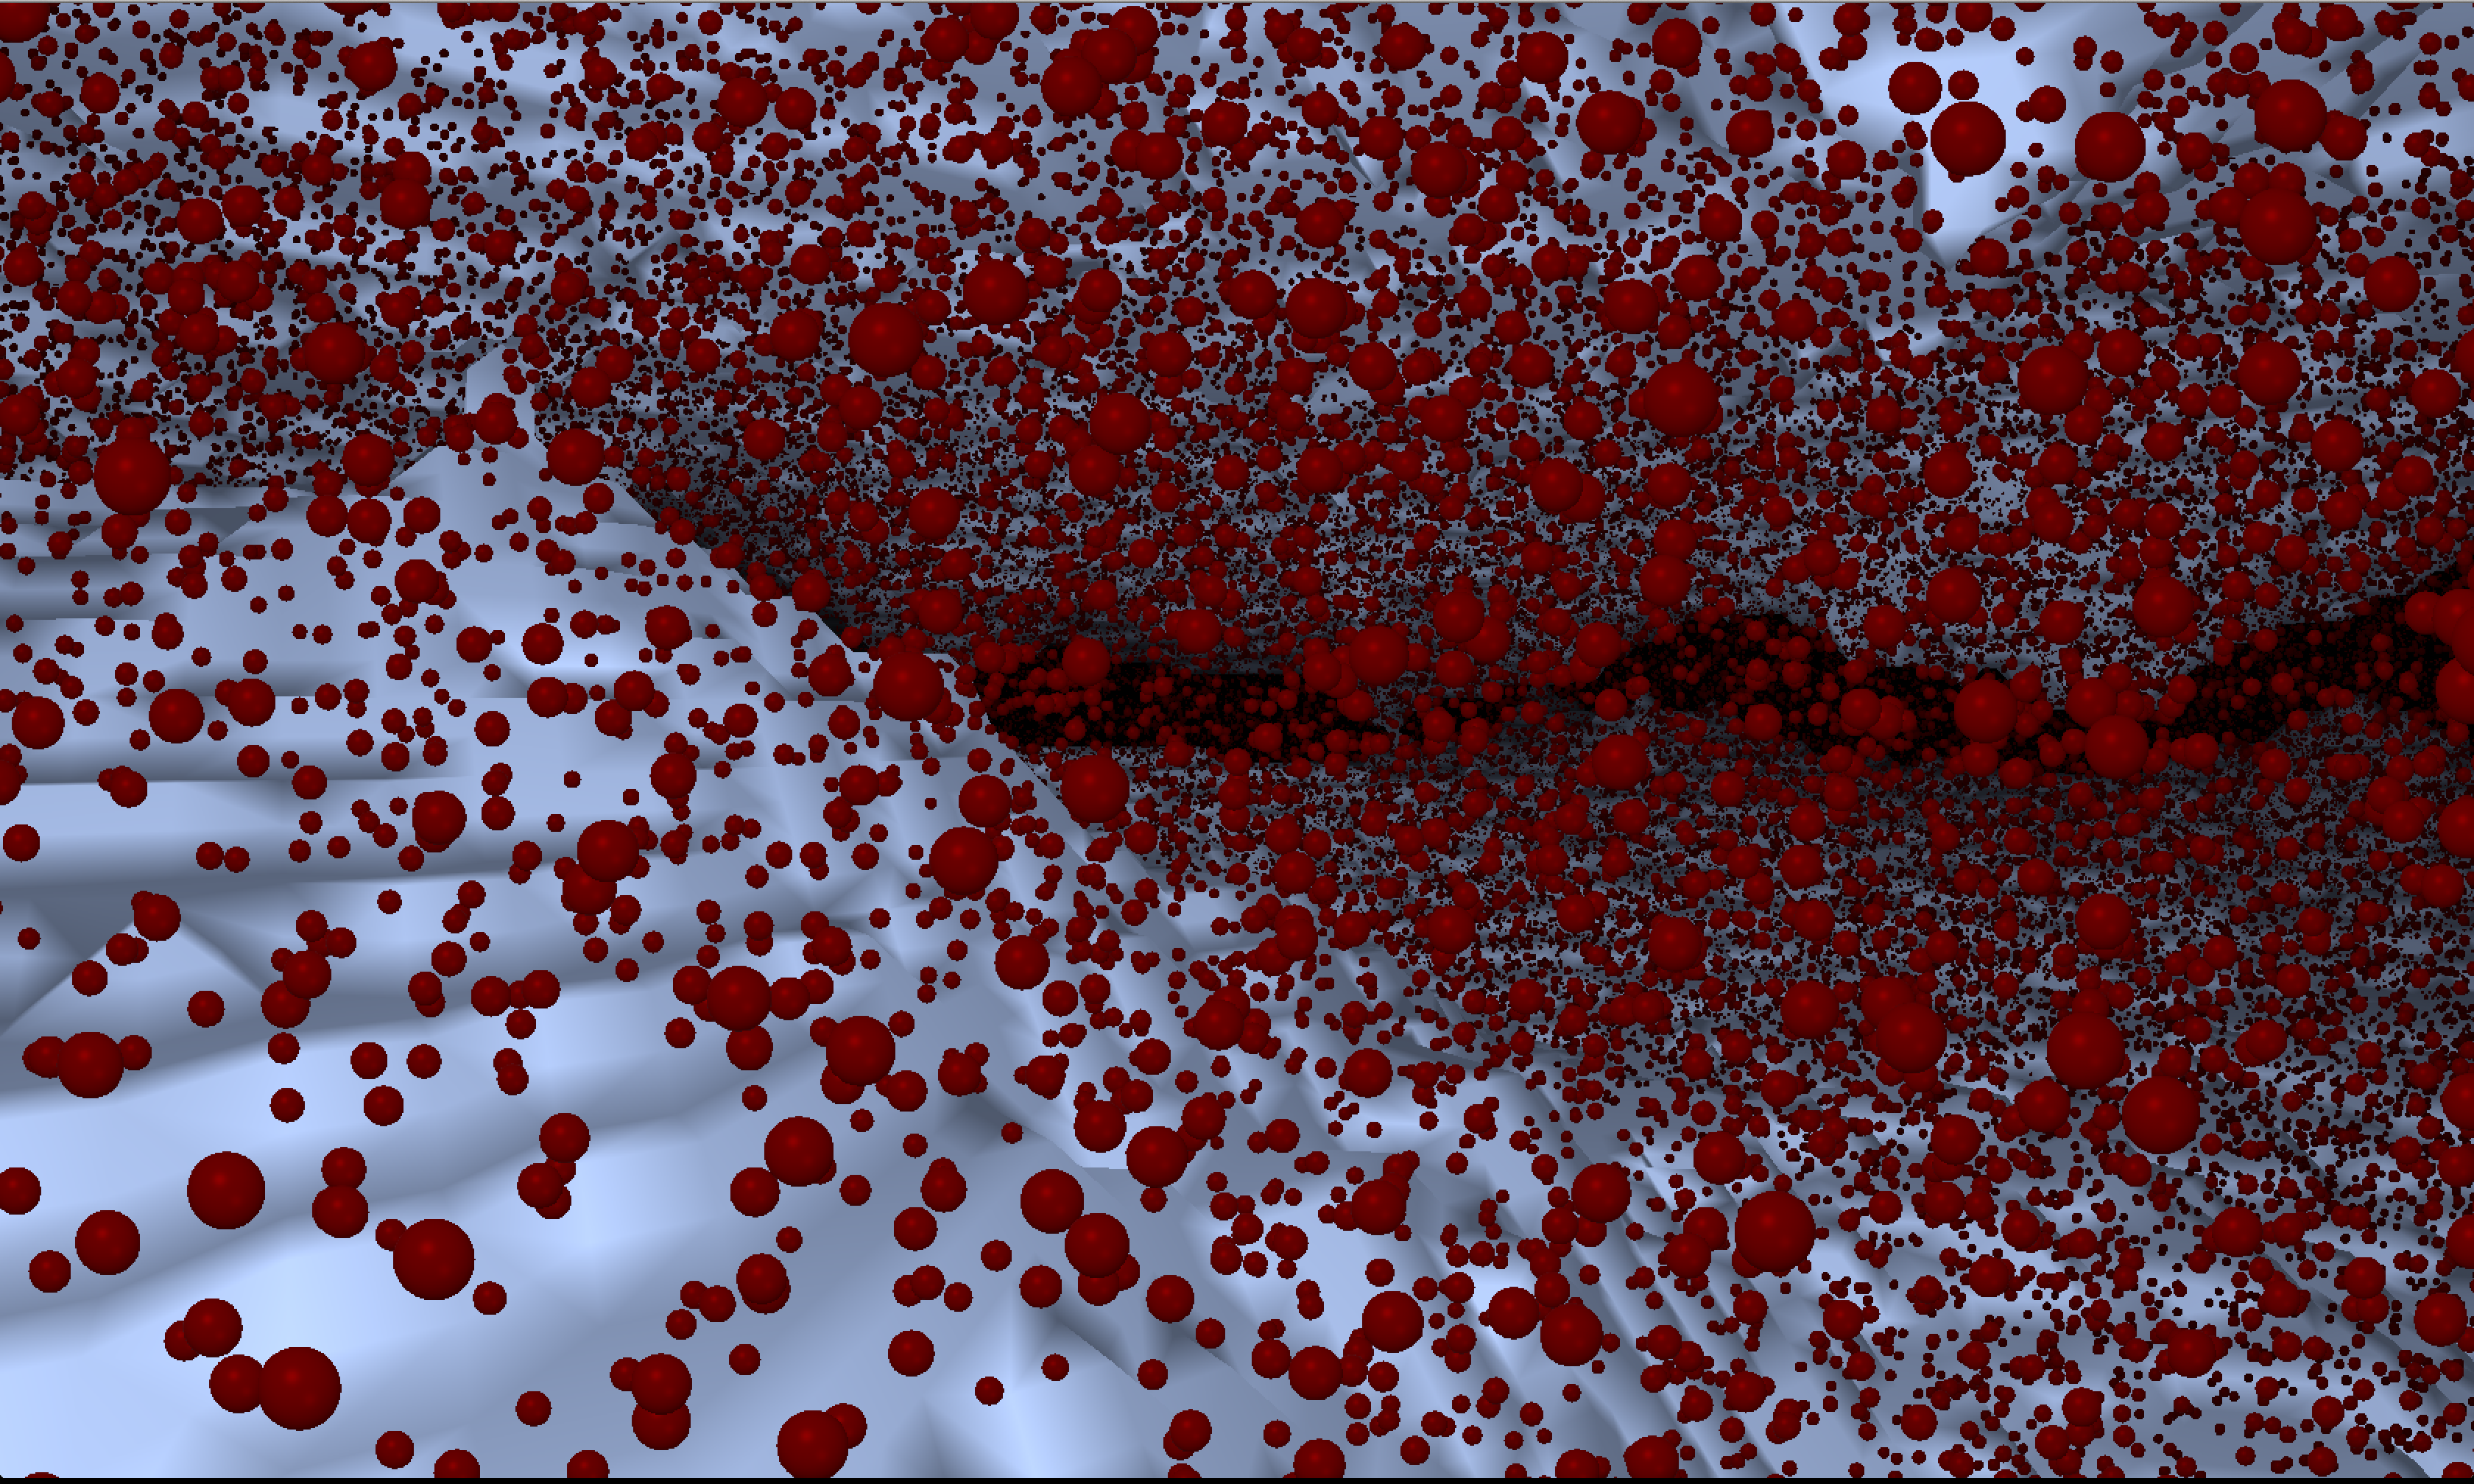
\includegraphics[width=\textwidth, trim=0cm 0cm 0cm 0cm, clip]{visualization/figures/marching_cubes_fracture.png}
\end{center}
\caption{Here we see a live simulation on a 2013 Macbook Pro. One million DSMC particles in a fracture created with the diamond-square algorithm (a thanks to Filip Sund who implemented this algorithm). With a good frame rate it is easy to study flow in any region of the system. }
\label{fig:vis_marching_cubes}
\end{figure}

\begin{figure}[htb]
\begin{center}
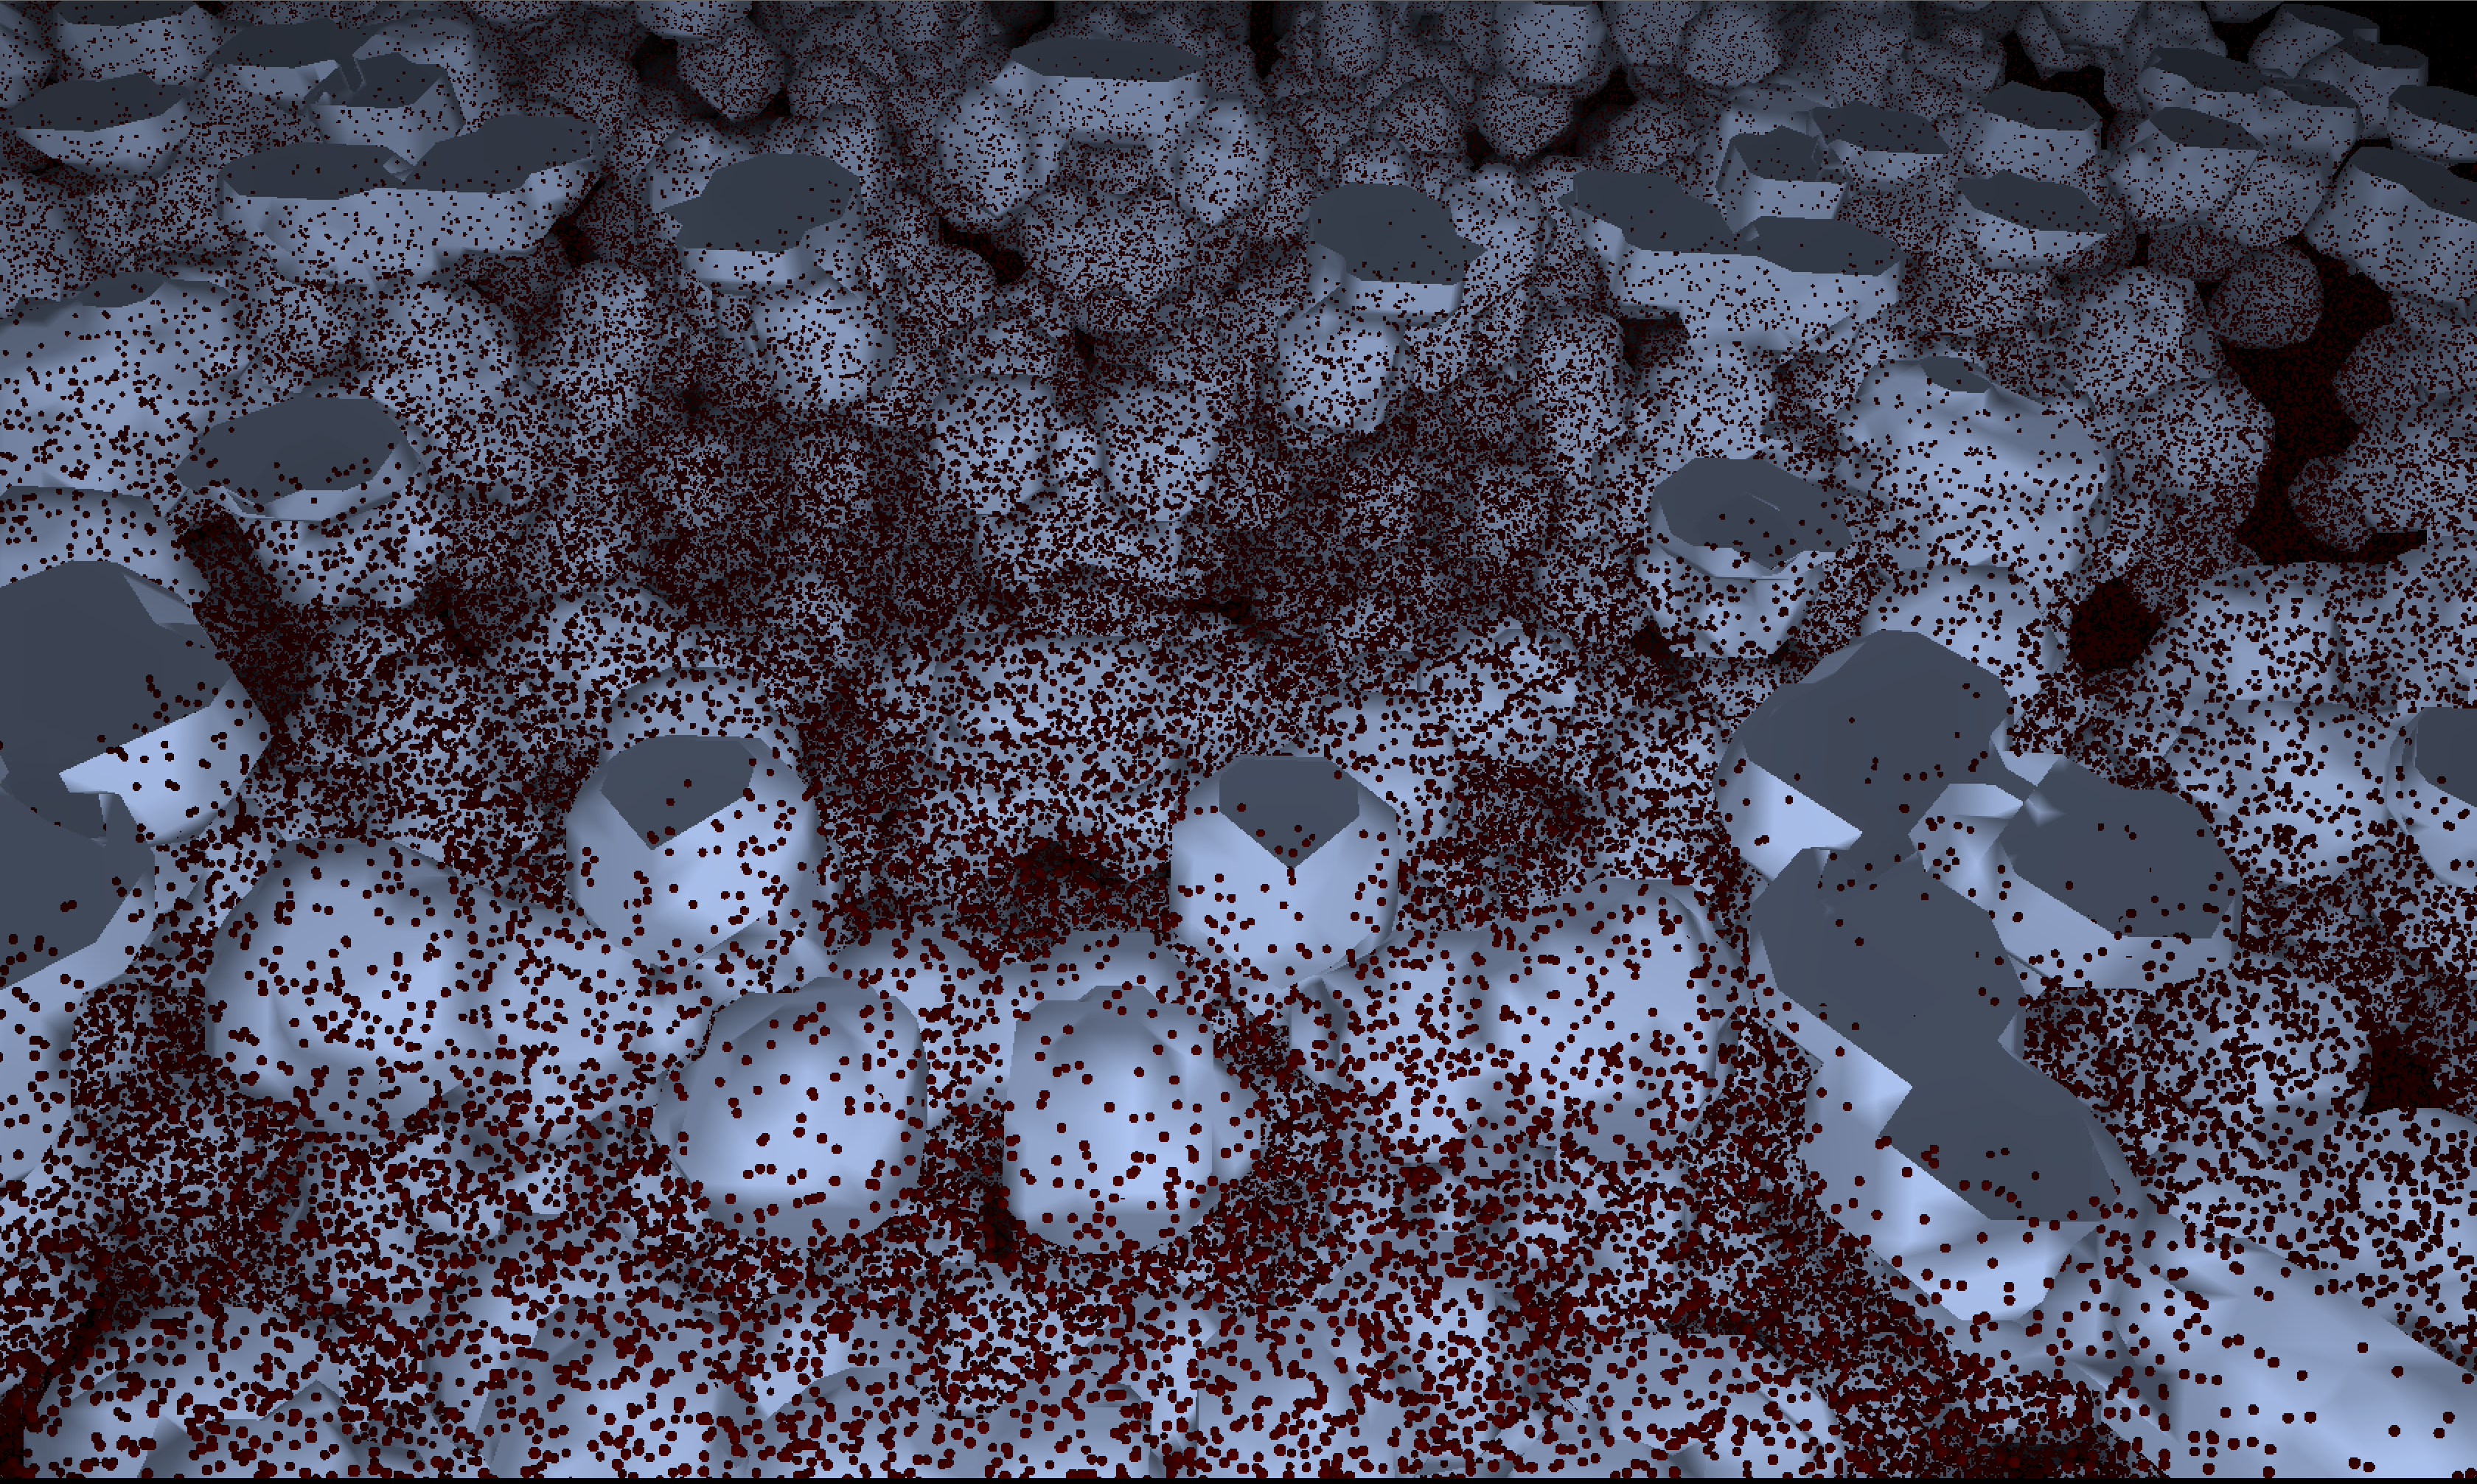
\includegraphics[width=\textwidth, trim=0cm 0cm 0cm 0cm, clip]{visualization/figures/marching_cubes_spheres_2.png}
\end{center}
\caption{This is a live simulation of four million DSMC particles in a system consisting of packed spheres.}
\label{fig:vis_marching_cubes_2}
\end{figure}

